\subsection{The simplex algorithm}

In corollary \ref{Cor:always_extreme_points} we saw that we can always find an optimal solution for an LP by looking at all the extreme points. The simplex algorithm is a method that enumerates them in order of decreasing cost. 

Recall that an LP is in standard form if

\begin{align*}
\min cx\\
Ax = b\\
x\geq 0
\end{align*}

and $A\in \R^{m\times n}$ has $m$ linearly independet rows. A \emph{basis} $B\subseteq [1,n]$ is as set of $m$ column indices such that $A_B$ has full rank $m$ (Note that $A_B$ can be inverted as the rows are linearly independet). It induces a \emph{basic solution} (see \ref{Def:BasicSolution} for a basic solution definition)

\[\begin{cases} x_B = A^{-1}_Bb\\ x_{\bar B} = 0\end{cases}\]

If $x_B$ is a basic solution, the variables $x_{B(1)},...x_{B(m)}$ are called \emph{basic variables}. The remaining variables $x_i|i \neq B(1),...,B(m)$ are called \emph{nonbasic}. 

We say it is feasible if $x_B\geq 0$. Note that the $x_{\bar B}=0$ part makes $n-m$ non-negativity constraints active so that we actually are at a corner with $n$ active constraints in $n$ dimensions.

In other words (the book):
\begin{enumerate} 
 \item Choose m linearly independet columns $A_{B(1)},...,A_{B(m)}$
 \item Let $x_i=0$ for all $i \neq B(1),...,B(m)$
 \item Solve the system of $m$ equations $Ax=b$ for the unknowns $x_{B(1)},...x_{B(m)})$
\end{enumerate}
The basic solution is given by the results of step three.

\paragraph*{Degeneracy}
Certain basic solution are degenerate. 
\begin{Def}[Degeneracy]
 A basic solution $x\in \R^n$ is said to be degenerated if more than $n$ of the constraints are active at $x$ 
\end{Def}
In 2D this means that more than two lines intersect at one point.

%das ist didaktisch hier fehl am platz
The interesting property is, that we can't get the same basic solution from two different bases, if we have a non-degenerate LP. In the degenerate case this may very well happen. Below examples shows the problem:

\begin{align*}
x_2 + x_3 &= 1\\
x_1 - x_2 +x_4 &=0\\
x_1 + x_2 +x_5 &= 2\\
\end{align*}

% figure

The above system gives us the solution $(1,1,0,0,0)$ for three bases $\{1,2,3\},\{1,2,4\},\{1,2,5\}$. This happens because we have a point where three constraints are active, although we're in 2D. See figure \ref{Fig:degenerateLP}. It is easy to see that if we have two bases build from indices $k\in [1,\ldots,n]$ that give us the same solution one of the $x_k$ (a basic variable) has to be zero. %easy to see :S

%figure
Note that degeneracy is not a purely \emph{geometric property} (representation independend). However if a basic feasible solution of a particular standard form representation of a polyhedron $P$ is degenerated, then it is degenerated under all standard form representations of $P$.


\paragraph*{The simplex algorithm} works by moving from corner to corner, always in the direction of better costs. At first we'll have some simplifying assumptions, to avoid the messy details:

\begin{enumerate}
\item The LP is in standard form (for conversion see \ref{Sec:standardForm})
\item Every feasible basis $A$ is non-degenerate. A basis $B$ is non-degenerate if $\forall b:\ x_B=A^{-1}_Bb \gneq 0$. Note the difference to $x_B\geq 0$ for general basic solutions. So it is forbidden that more than $n$ (those in $B$ and $>n-m$ non-negativity) constraints are active (in $n$ dimensions they can't all be linearly independet of course). 
\item We are given an initial feasible basis
\item The feasible region of the LP is bounded
\end{enumerate}

In the next lectures we'll remove those assumptions one after the other.

An initial version of the algorithm works as follows:
\begin{center}
\begin{lstlisting}
SIMPLEX-TAKE-I(A,b,c)

B <- find some feasible basis
// B=$\{b_1,b_2,\ldots, b_m\} \subseteq [1,\ldots, n]$
repeat 
    for $j\in [1,n]\backslash B$ and  $b_i \in B$
        D = B $\cup$ j $\backslash$ $b_i$
        if D is a basis then
            $x_B$ = $A^{-1}_B$b
            $y_D$ = $A_D^{-1}b$ //a basic solution
            if ($y_D$ $\geq$ 0) //a bfs
                if($c_Dy_D < c_Bx_B$) //cheaper than $B$
                    B = D
until B hasn't changed                
\end{lstlisting}
\end{center}

We switch from a basis $B$ to a basis $D$ by removing a column $b_i$ from $B$ and putting in a replacement $j$ to get back to a (hopefully) full rank matrix $D$. We then check if $D$ is non-singular. If so it induces a basic solution, we just have to check if it's feasible. If yes we check if the cost of the new induced solution $y_D$ is better that the old $x_B$ and keep $D$ if it is an improvement.

It will later turn out that we don't actually have to check every combination for $j$ and $b_i$. The choice of $b_i$ is uniquely determined by the choice of $j$.



When we move from solution $x$ to solution $y$ we do so along some vector $d$ (s.t. $y=x+\Theta d$). Have a look at figure \ref{Fig:movingToSolutions}. We do some observations on the vector $d=(x_0,...,x_n)$. $d_k$ refers to the k-th component of $d$. 

\begin{figure}[hbt]
\begin{center}
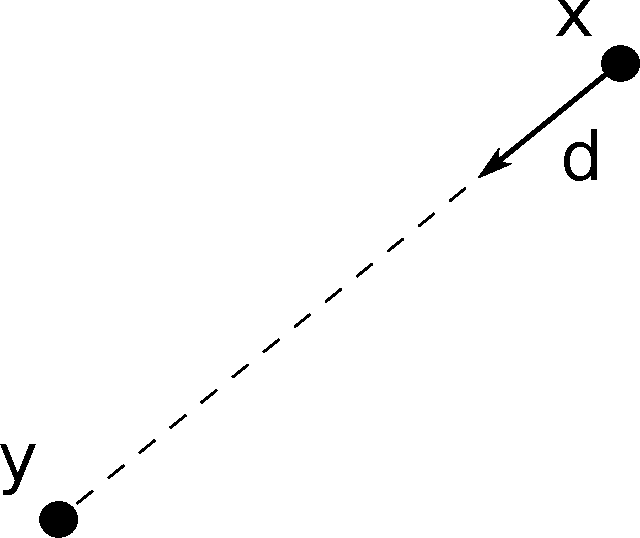
\includegraphics[width=0.3\textwidth]{./images/movingToSolutions.pdf}
\end{center}
\caption{The vector $d$ gives the direction from $x$ to $y$.}
\label{Fig:movingToSolutions}
\end{figure}


\begin{itemize}
\item $d_k=0$ if $k\not \in B \cup j$, because we assumed all non-basic variables to be zero to make the non-negativity constraints active. In particular the column $b_i$ is removed from the basis and hence the variable $x_{b_i}$ becomes $0$.

\item $d_j>0$ let $j$ be the column added to the basis, because we made the formerly non-basic variable $x_j$ basic. That is assigning it some value $>0$. By choosing $\Theta$ accordingly we can scale this to be $d_j=1$ and make further calculations easier. Therefore we assume from now one $d_j=1$

\item $Ad = 0$ because both $x$ and $y$ are bfs, i.e. both satisfy all equations: $Ad = (Ay-Ax)/\Theta = (b-b)/\Theta = 0$
\end{itemize}

By using these observations we can directly calculate the $b_i$ we need to remove.

First we want to get the components $d_B$ that we don't know immediately from the above observations. We can decompose $Ad$ into the part we're looking for, $A_j d_j$ which is $A_j$ since $d_j:=1$ and $A_{\bar B} d_{\bar B}$ which is 0 since $d_{\bar B}:=0$. $B$ is a basis, so $A_B$ is invertible and we can compute $d_B$.

\[Ad = A_B d_B+A_j = 0 \Rightarrow d_B = -A^{-1}_B A_j\]

The new extreme point $y$ should be a feasible solution so we also want $y\geq 0$. By plugging in the calculation for $d_B$ into the equation for the line between $x$ and $y$ we get

\begin{align*}
y_B &= x_B + \Theta d_B\\
 &= x_B + \Theta A_B^{-1} A_j\\
 &= x_B - \Theta A_B^{-1} A_j \geq 0
\end{align*}

Remember that the basic variables in $x_B$ are all greater than 0. So that means if $d>0$ we are ok, however if for some $b_i$ $d_{b_i} <0$ then it can happen that we get a negative component if we choose $\Theta$ too large. We need 

\begin{align*}
x_{b_i} +\Theta d_{b_i} &\stackrel{!}{\geq} 0\\
\Theta &\leq \frac{-x_{b_i}}{d_{b_i}}
\end{align*}

By choosing $\Theta$ sufficiently small we can avoid negativity. However we'd like to move as far as possible along the line $y=x+\Theta d$ without leaving the polyhedron. So we choose it like this

\[\Theta = \min_{{b_i\in B}\atop {d_{b_i} <0}} \left| \frac{x_{b_i}}{d_{b_i}}\right |\]

The variable $x_{b_i}$ that attains the above minimum will be equal to zero in $y$, i.e. in becomes non-basic and will have to be taken out of $B$. Because we assumed that the system is non degenerate there will be only one element actually attaining it or we would have a basic feasible solution with a basic variable that is 0 (and hence $>n$ constraints would be active at that solution). Also $\Theta \gneq 0$ or one of the basic variables would have been zero ($\Rightarrow x\neq y$).

Note that this was the step that assumed a bounded polyhedron. If $d>0$ we can move along $x+\Theta d$ as far as we want without leaving $P$. So $P$ contains a line and is not bounded (remember figure \ref{Fig:bounded_unbounded}).

Next we want to look at how the cost changes when going from $x$ to $y$. Again we do this by plugging in our observations into the line equation:

\begin{align*}
cy &= cx + \Theta cd\\
    &= cx - \Theta (c_B(A_B^{-1} A_j) + c_jd_j)\\
    &= cx - \Theta (c_B(A_B^{-1} A_j) + c_j)\\
cy - cx &= \Theta (c_j - \trans c_B A_B^{-1}A_j)
\end{align*}

If $y$ was a solution that we move to we did that because $cy$ was smaller that $cx$. So $c_j - c_B^TA^{-1}_B A_j$ should be negative if we want to move to $y$.

Now we know how to calculate the $b_i$ we need to remove when we put in a $j$ to get a new basis and we know a new (much more complicated, yay) criterion to check whether we move in the right direction. We combine that into a better version of the algorithm.

\begin{center}
\begin{lstlisting}
SIMPLEX-TAKE-II (A,b,c)

B = some feasible basis
repeat 
    for $j\in \{1,\ldots,n\}\backslash B$ // $b_i$ is determined
        $d_B$ = $A^{-1}_B A_j$
        if $c_j - \trans c_BA^{-1}_B A_j < 0$
            $b_i$ = index  s.t. $d_{b_i} <0$, 
                    minimizing $\left| \frac{x_{b_i}}{d_{b_i}}\right|$
            B = B $\cup$ j $\backslash$ $b_i$
until B hasn't changed
\end{lstlisting}
\end{center}


\begin{center}
\begin{lstlisting}
SIMPLEX-TAKE-III (A,b,c)

B = some feasible solution
repeat
    $\bar c$ = $c_j$ - $\trans c_B A^{-1}_BA$ //reduced cost vector
    if $\exists j:{\bar c}_j<0$ 
        u = $A^{-1}_B A_j$ // dimension m
        $b_i$ = index in B s.t. $u_i >0$ 
                minimizes  $x_{b_i}/u_i$
        B = B $\cup$ j $\backslash b_i$ 
until B hasn't changed 
// $\bar c \geq 0$ 
\end{lstlisting}
\end{center}

The algorithm always terminates because the assumptions ensure that we always have a optimal solution and we improve our solution in every step.

\begin{thm}\label{Pr:simplexIIIopt} Let B be a basis. If $x_B=A^{-1}_Bb\geq 0$ and $\bar c=c-\trans c_B A_B^{-1}A_j$ then $B$ is optimal.\end{thm}

\begin{pr}[Theorem \ref{Pr:simplexIIIopt}] Let $x$ be the bsf induced by $B$, $y$ be some feasible solution. We want to argue that the cost of $x$ is smaller than the cost of $y$. Let $d=y-x$ then 
\[cd = c_Bd_B + \sum_{j\in \bar B} c_jd_j \] 

To be continued
\end{pr}